\documentclass{article}
\usepackage[utf8]{inputenc}
\usepackage[a4paper, margin=2cm]{geometry}
\usepackage{indentfirst}
\usepackage{graphicx}
\usepackage{hyperref}
\usepackage{csquotes}
\usepackage{subfig}
\usepackage{color}

\title{Uliège eShop \\e-commerce and e-business project}
\author{Beguin Mathias - Lejoly Loic \\ Github access: \url{https://github.com/MTHSBGN/e-commerce}}
\date{November 2018}

\begin{document}

\maketitle
\newpage

\section{Introduction}
For this project, we decided to work on the proposition given in the statement (Uliège eShop). As asked in the statement the goal is to provide a website where objects related to the University can be sold. To achieve that, we decided to use a relational database to store products and data related to customers. Concerning the back-end's website \textit{Node.js} and SQL are used. \textit{Node.js} is a cross-platform JavaScript run-time environment. That means JavaScript is used outside client browser. This cross-platform is young compare to PHP but more and more companies tend to use it due to its design and its scalability. Concerning the front-end part as usual HTML,CSS and JavaScript are used.

\section{Database architecture}
To model the database of the Uliège eShop website a relational database architecture was chosen. The reason of this choice is justified by the product catalogue is not large and because it can be hard to have a good NO-SQL design. On the web you can find some debates that discuss the fact to use relational DBs or no-SQL DBs. The advantage of the no-SQL DB is that it is easier to manage your product catalogue (product variations) but the drawback of no-SQL DBs is the reliability (can be solved with DB clustering e.g: foundationdb, couchDB,...). Concerning the reliability relational DB architectures are, for the majority, ACID compliant. These two types of architectures are not mutual exclusive. Most of the time, e-commerce websites use of combination of SQL and No-SQL DBs (a paper discussing that topic \url{https://aisel.aisnet.org/cgi/viewcontent.cgi?article=1026&context=sais2013}).

\subsection{entity-relationship model}
\autoref{ecommerce_er} depicts the entity-relationship model based on the minimal requirements given in the statements. We decided to split the product table proposed in the statement into multiple tables to avoid data replications and to provide a scalable approach. Indeed, in the product table proposed, all data linked to a product is packaged into this table. The result of that is it is difficult to manage products with different properties (e.g colors, size,...) without replications. That is why we decided to split this table into several tables that are \textit{Sku (stock keeping units) Variant (gives the properties of a product), Image(image paths related to a product), Description (Give the product description), and Category (specify the product category)}. \\

Concerning the transaction part we decided to split that part into two related steps. The first step establishes a relation between the sku ID, the order ID (defined in the second step) the  current price of the product during the order and the quantity needed. This step is achieved with the table Order\_details. The second step consists in summarizes the the order of the client by referencing the ID of the order, the delivery address, the total price of the order, and  the user ID.

\subsection{Relational model}
\begin{enumerate}
\item Customer(client\_id, mail, username, password, delivery\_address, firstname, lastname, cookie\_id)
\item Client\_order(order\_id, \#client\_id, date, total\_price, ship\_address)
\item Order\_details(\#order\_id, \#sku\_id, quantity, price)
\item Product(product\_id, \#category\_id, \#image\_id, \#description\_id, name)
\item Image(image\_id, \#sku\_id, filename)
\item Sku(sku\_id, \#produt\_id, price, available, sold)
\item Variants(variant\_id, attribute, value)
\item Description(description\_id, french, english)
\item Category(category\_id, \#description\_id, name)
\end{enumerate}

\begin{figure}[h!]
    \centering
    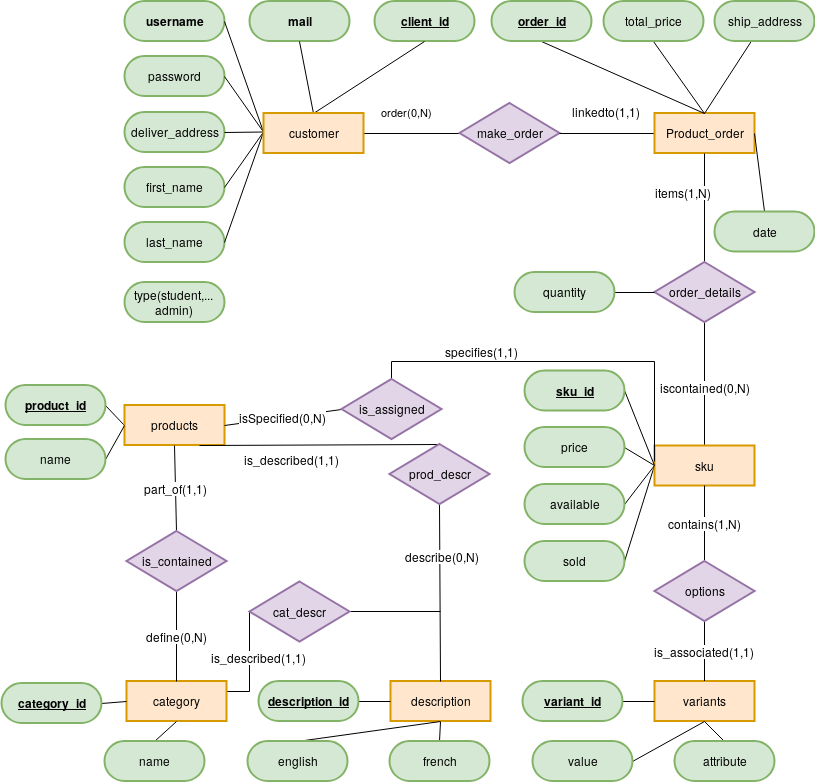
\includegraphics[scale=0.4]{./images/ecommerce_ER.png}
    \caption{eShop entity-relationship model}
    \label{ecommerce_er}
\end{figure}

\subsection{model to SQL tables}
The entity-relational model depicted on \autoref{ecommerce_er} can be translated into SQL tables as \autoref{ecommerce_sql} shows. If you want a more interactive view of these tables, you can load the SQL file in \textit{phpmyadmin} for instance.

\begin{figure}[h!]
    \centering
    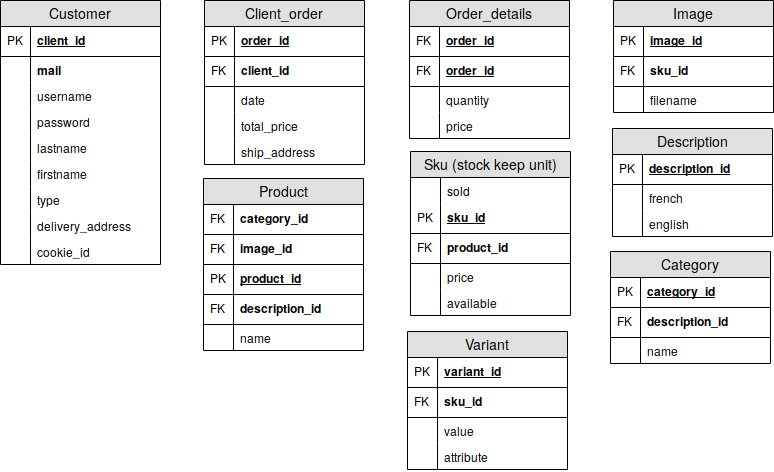
\includegraphics[scale=0.4]{./images/ecommerce_SQL.png}
    \caption{eShop entity-relationship model}
    \label{ecommerce_sql}
\end{figure}

\section{Website}
The website is divided into section. The first section is dedicated to the admin of the website itself. This panel can only be accessed by users with the right privileges. The second second is dedicated to customer where they can buy products. For the development of the website we applied minimal protections like SQL injection managed by the \textit{Node.js} server.

\subsection{Admin panel}
The admin panel is a dashboard provided to the administrator of the website. The users that can use this panel have special privileges. To detect this kind of users the field \textit{type} of customer table is set to zero. As results, a admin user needs to follow the regular registration phase to create an account and then the super user that has a direct access to the database can change the \textit{type} field to promote a user as admin user. Admin users have an extra button to allow them to access to the admin panel.\\

The dashboard is simple, at left a menu can help the user to navigate through the different webpages. As you can see on the \autoref{fig:admin} the panel only contains 3 pages \textit{(home,product,category)}. The homepage summarizes different parameters, you can also export some data. The product and category pages give the possibility to add new elements to the database easily. \\

Even if you are on the dashboard you can go back to the e-commerce pages just by clicking on the website button.

\begin{figure}[h!]
    \centering
    \subfloat[admin homepage]{{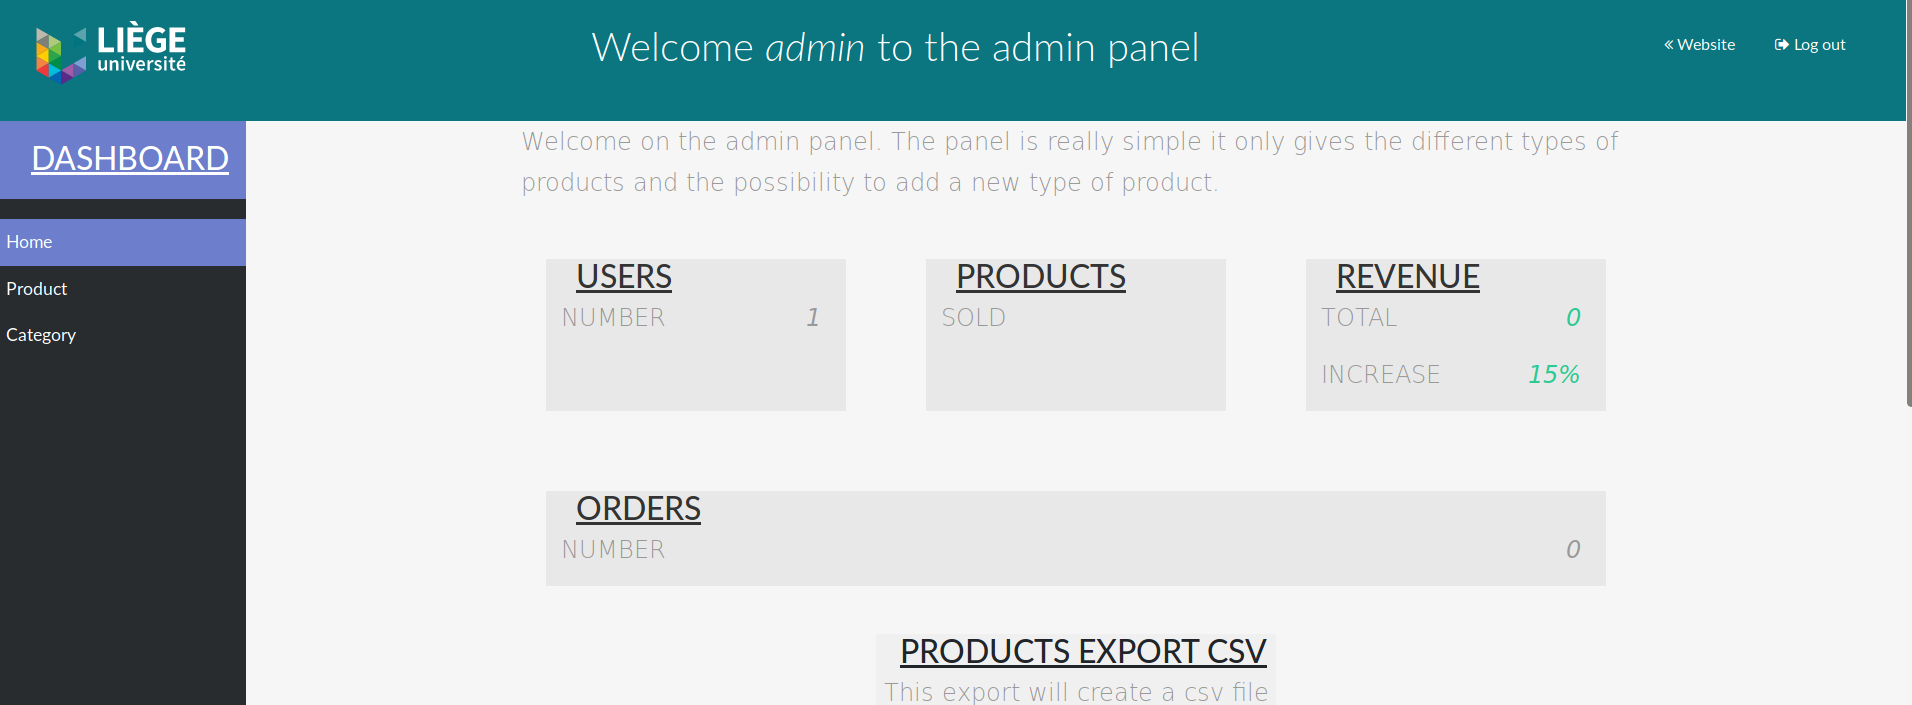
\includegraphics[scale=0.2]{./images/index_admin.png}}}%
    \qquad
    \subfloat[product manager]{{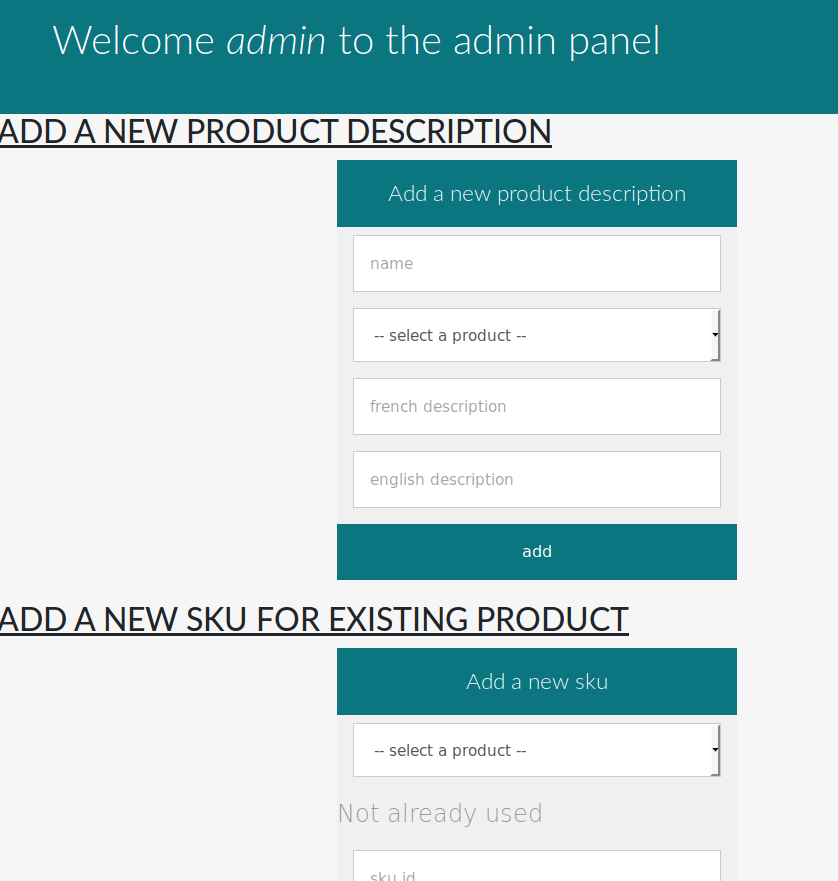
\includegraphics[scale=0.3]{./images/product_admin.png}}}%
    \caption{admin pages}%
    \label{fig:admin}%
\end{figure}

\subsection{Customer View}
If you are a regular customer, you can just have access to the e-commerce webpages. On the homepage you can see the different products that are sold by the University. On top of the website at right you have several buttons. One to create an account, one to have access to your basket and one which is the about page. To buy products a user needs to create an account and this account must be active.\\

A user can scrolls the homepage that contains all products and when he is interested by a product, he can click on that product and he will be redirected that the detailed product page.\\

Like common e-commerce websites, users can search for products by using search-bar or simply by walking through the website. Concerning this website, we do not received enough information concerning products (i.e: categories, etc.) so we decided to display categories since the number of products to display is rather small. Nonetheless, products has a category as you can see on the database schema. Administrators have thus the choice to use it or not.

\subsubsection{Registration}
To purchase products, a customer needs to create an account on the website to do so, he needs to click on the button dedicated to that purpose or simply follow the appropriate url. On that page the user must fill fields with correct informations and then validate his account. If everything is correct, he is redirected to the login page.
 
\subsubsection{Log in}
After the creation of an account, a user can connect to the website by using his account information. To achieve that he simply clicks on the button made for that purpose or is going to the appropriate url. If information given is correct he will be redirected on the homepage.

\begin{figure}[h!]
    \centering
    \subfloat[register page]{{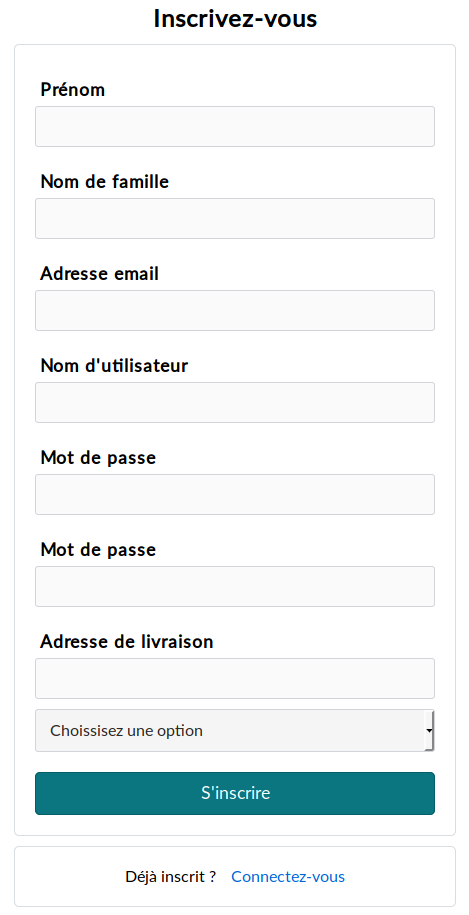
\includegraphics[scale=0.3]{./images/sign_up.png}}}%
    \qquad
    \subfloat[login page]{{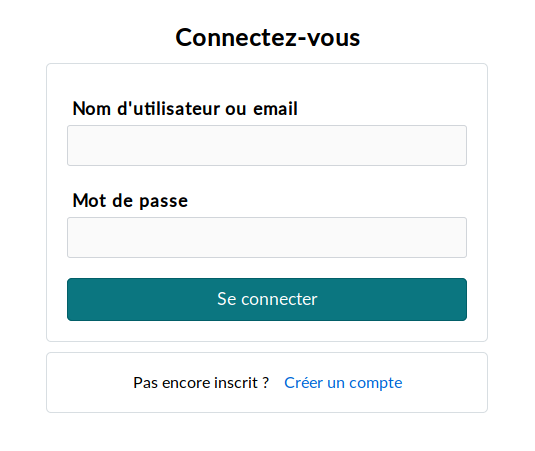
\includegraphics[scale=0.3]{./images/sign_in.png}}}%
    \caption{connection pages}%
    \label{fig:mineral}%
\end{figure}

The login page is the same for the admin, since the admin has more privileges when he is logged, he can access more pages such has the admin panel.

\subsection{Basket}
To store the basket of a user, HTTP cookies are used. When a user clicks on its basket, he obtains a summary of his products. This summary gives the possibility to modify product quantities or to delete some of them. When the user is in accordance with his order summary, he can validate it only if he has an account and if he is connected. The validation process send information to the payment procedure where all element are stored and where the order becomes effective.

\subsubsection{Payment}
Since none payment procedure like PayPal etc. is set for this project, a simple payment page is used to update the database. Even if it is a simple page, a transactional commit phase is established to be sure that all tables are updated correctly.

\subsection{Security aspects}
Concerning the security of the website, some common guidelines are applied such as SQL injections and transactional commits. But to provide a robust website some other security rules must be applied such as directory permissions, redirection rules by catching different errors,...

\section{Market model}
Concerning the target of the website it is obvious. It concerns essentially Alumni, employees and students of ULiège. The eShop provides a bunch of goodies related to the university and the city of Liège. Prices given are affordable for student and the aim of the eShop is not to be competitive with others websites that sell similar products. The aim is to provide a website where university community can buy university products easily. The website can also be used by student associations to sell their pulls for instance an provides a legal framework to sell them.

\section{Improvements}
Concerning the website some improvements can be done. First of all concerning the design, we tried to have a flat design user interface but we are not web designer nor user experience designer (UX). After that, security aspects must be improved and not neglected (DDoS attacks,XSS,etc.).
\end{document}

